	Le dashboard étant maintenant terminé, une phase de recette a été organisée avec deux métiers ainsi que mon chef de projet afin que je puisse présenter le travail que j'avais effectué. Des extraits sont disponibles en annexe \ref{c2}. Tous les graphiques ont été passés en revue et les métiers ont pu vérifier que chacun des besoins que je m'étais engagé à satisfaire était effectivement présent sur ledit dashboard. Au terme de cette réunion, le dashboard a été approuvé malgré les quelques spécifications qui n'avaient pas pu être satisfaites et nous avons donc décidé de le mettre en place sur tous les environnements à savoir Homo3, RGB et la production. Nous avions déjà schématisé ces environnements figure \ref{environnement} mais ces derniers étaient incomplets. En effet, en réalité, chacun d'entre-eux possède différentes VM dont une dite de \textit{supervision} contenant les outils de monitoring et de supervision et une appelée \textit{microservice} sur laquelle se trouve le code source de l'API microservices. Les environnements RGB et de prod possèdent même deux VM microservices pour le load-balancing. La stack ELK a été installé sur supervision alors que FileBeat a été installé sur microservices (a et b) puisqu'il devait récupérer les logs générés par l'API. J'ai eu la chance de pouvoir procéder moi-même à l'installation de tous les éléments sur RGB. Après cela, je me suis occupé de la maintenance de ces outils afin de corriger les éventuels problèmes qui apparaissaient.\\
	
\begin{figure}[h!]
	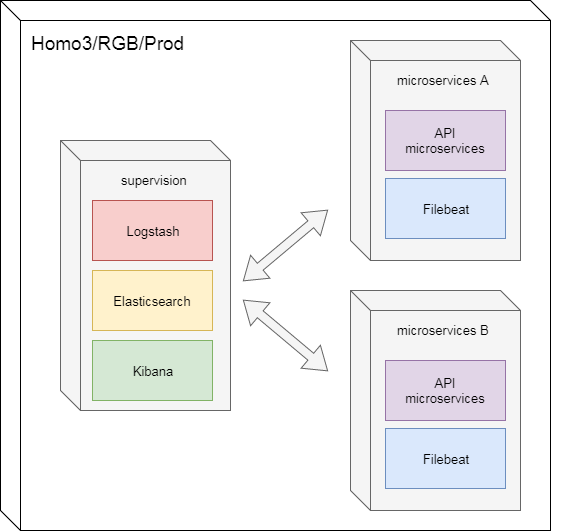
\includegraphics[scale=0.5]{images/travailNeuflizeOBC/dashboard/elkDeploiement.png}
	\centering
	\caption{Architecture de la stack ELK sur tous les environnements}
	\label{elkDeploiement}
\end{figure}